\newcommand{\vocab}{\mathbf{v}}
\newcommand{\dtvec}{\mathbf{t}_\Delta}
\newcommand{\ctxvec}{\mathbf{t}_\text{ctx}}
\newcommand{\dt}{\Delta_t}
\newcommand{\prerror}{Pr_{error}}
\newcommand{\weights}{\mathbf{w}}
\newcommand{\X}{\mathbf{X}}
\newcommand{\post}{\rho}
\renewcommand{\t}{t}
\newcommand{\w}{w}
We aim to predict the amount of time between the arrival of the next post and 
the time the last post in the thread was made. The information available to us 
are the previously made posts that we observe when first visiting the thread.  
The assumption made here is that the thread is not paginated in any way, and a 
single visit to the thread gives us the latest posts without having to traverse 
through the links to the latest page. This is because in practice, we would be 
able to keep track of where the last visited page of the thread was, and reading 
the new posts would incur a few more requests to the thread. This, in comparison 
to constantly hitting the page for updates, would be negligible.

More formally, what we are trying to do is to estimate a function $f$ such that 
given a feature vector $\X$ representative of a window $\post_{t - w + 
1},\post_{t - w + 2},\cdots ,\post_t$, where $\post_t$ represents the $t$-th 
post in the thread, we can approximate $\dt$ with $f(\X)$.  In the following 
sections, we will discuss various methods for estimating $f$.  Various notations 
will be used, a quick reference is provided in Table \ref{table:notations}.


\begin{table}
	\begin{center}
	\begin{tabular}{l l}
	\hline
Notation	&	Description\\
	\hline
$\post$		&	A post\\
$\t$		&	Index of a post in a thread\\
$\w$		&	Number of posts in a window  \\
$\post_\t$	&	The $t$-th post in the thread\\
$\vocab_\t$	&	The frequency count vector of the posts used in the $t$-th 
	post\\
$\dt$		&	Time difference between a post at position $\t$ and a post at 
	position $\t+1$ \\
$\dtvec$	&	Vector of $\dt$s in a given window\\
$\ctxvec$	&	Bit vector representing the day of week, and the hour of day\\
$\X$		&	Feature vector extracted from a window\\
$K$			&	The $K$ best features selected from the vocabulary.\\
	\hline
	\end{tabular}
\end{center}
\caption{Notation reference} \label{table:notations}
\end{table}


In the following sections, we describe the various methods we have to 
approximate $f$.

\section{Baselines}
A simple way of estimating the revisit rate would be to use the average time 
differences given the observed posts, or a training set. In previous work, we 
have seen that if page updates follow a Poisson distribution, then revisiting at 
the Poisson mean would be an optimal revisit policy. %cite paper

In our baseline revisit policy, we took into account the last made post whenever 
we make a visit to the thread, and calculate our next revisit time based on the 
average post intervals added to the timestamp of the previous post. This is in 
contrast to an even simpler revisit policy that just revisits at a constant, 
fixed rate, independent of the posts being made to the thread.

One other way of predicting using average post intervals would be to use the 
concept of a \emph{window}. Averaging out the time differences between the posts 
would intuitively work, because it captures the context of the situation: A 
series of posts with short intervals should mean that the next post would come 
at around the same interval as the few that came before.

In terms of using content for prediction, windows also make sense: Forum users 
view content as paginated posts, so time differences between posts do not affect 
their decision to post. Rather, reading a number of posts together affect 
whether or not the user chooses to reply.

An example of a window ($w=2$) can be seen in Figure \ref{fig:event_series}.

\begin{figure}
	\begin{center}
	
\tikzstyle{background}=[rectangle,
	fill=gray!10,
	inner sep=0.2cm,
	rounded corners=5mm]


\tikzstyle{post}=[circle,
	thick,
	minimum size=1.2cm,
	draw=blue!80,
	fill=blue!20]
% The measurement vector is represented by an orange circle.
\tikzstyle{visit}=[circle,
	thick,
	minimum size=1.2cm,
	draw=orange!80,
	fill=orange!25]

\begin{tikzpicture}[>=latex,text height=1.5ex,text depth=0.25ex]
    % "text height" and "text depth" are required to vertically
    % align the labels with and without indices.
  
  % The various elements are conveniently placed using a matrix:
  \matrix[column sep=0.3cm] {
    % First line: Control input
    	&
		\node (e0)					{};&
		\node (e1)	[post]			{};&
		\node (e2)	[visit]			{};&
		\node (e3)	[post]			{};&
		\node (e4)	[visit]			{};&
		\node (e5)	[post]			{};&
		\node (e6)	[visit]			{};&
		\node (e)					{};&
		&
        \\
	};
    
    % The diagram elements are now connected through arrows:

	\path[-]
		(e0) edge[thick]	(e1)
		\foreach \e in {1,2,3,4,5}{
			let \n1={int(\e+1)} in (e\e) edge[thick] (e\n1)
		}
		(e6) edge[thick]	(e)
	;

	\begin{pgfonlayer}{background}
		\node [background,fit=(e1) (e3)] {};
	\end{pgfonlayer}

\end{tikzpicture}


\begin{tikzpicture}[>=latex,text height=1.5ex,text depth=0.25ex]
    % "text height" and "text depth" are required to vertically
    % align the labels with and without indices.
  
  % The various elements are conveniently placed using a matrix:
  \matrix[column sep=0.3cm] {
    % First line: Control input
    	&
		\node (e0)					{};&
		\node (e1)	[post]			{}; &
		\node (e2)	[visit]			{}; &
		\node (e3)	[post]			{}; &
		\node (e4)	[visit]			{}; &
		\node (e5)	[post]			{}; &
		\node (e6)	[visit]			{}; &
		\node (e)					{};&
		&
        \\
	};
    
    % The diagram elements are now connected through arrows:

	\path[-]
		(e0) edge[thick]	(e1)
		\foreach \e in {1,2,3,4,5}{
			let \n1={int(\e+1)} in (e\e) edge[thick] (e\n1)
		}
		(e6) edge[thick]	(e)
	;

	\begin{pgfonlayer}{background}
		\node [background,fit=(e3) (e5)] {};
	\end{pgfonlayer}

\end{tikzpicture}

	\caption{%
A series of events, posts (blue) and visits (orange).  The diagram demonstrates 
the concept of a window of $w=2$.
}\label{fig:event_series}
	\end{center}
\end{figure}


\section{Performing regression on windows}
% Jesse: I dont understand what role this paragraph plays. It doesnt seem to
% add to explaining your method, which up to this point, still has not been
% explained.
% Shawn: To explain why I didn't do simple linear regression.
Previous work has used linear regression on a number of different features 
extracted from forums \cite{Yang2009}. In their paper, the regressed function 
was used as a scoring function rather than a predictive function. In site of 
this, we attempted to implement the same model, but this resulted in evaluations 
worse than that of the baseline.

We did use some of the features mentioned in the paper: Window posts time 
differences and time context features (bit-vector representations of the day of 
the week and hour of the day). In our own statistics we took from the 
\url{avsforum.com} threads, we have also found that the time of the day the day 
of the week matters when dealing with threads. An example of such a thread can 
be seen in Figure \ref{fig:hr_freq} and Figure \ref{fig:week_freq}, where it can 
be seen that activity on the board is highest at 2 PM, and drops slightly, 
suggesting some type of lunch period, and then goes up again during the early 
evening and at 9 PM, before dropping to its lowest at 3 AM. The weekly graph 
also shows a pattern, showing lower posting frequencies during the weekends, and 
its highest during Thursdays.
\begin{figure}
\begin{center}
\begin{subfigure}[b]{0.45\textwidth}
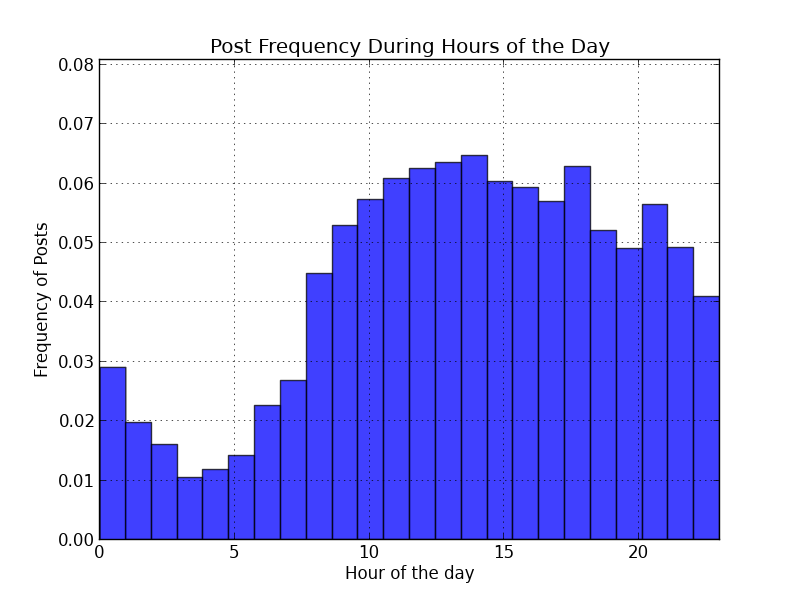
\includegraphics[width=\textwidth]{diagrams/hoursofday.png}
\caption{The hourly post frequency.}
\label{fig:hr_freq}
	\end{subfigure}
	\begin{subfigure}[b]{0.45\textwidth}
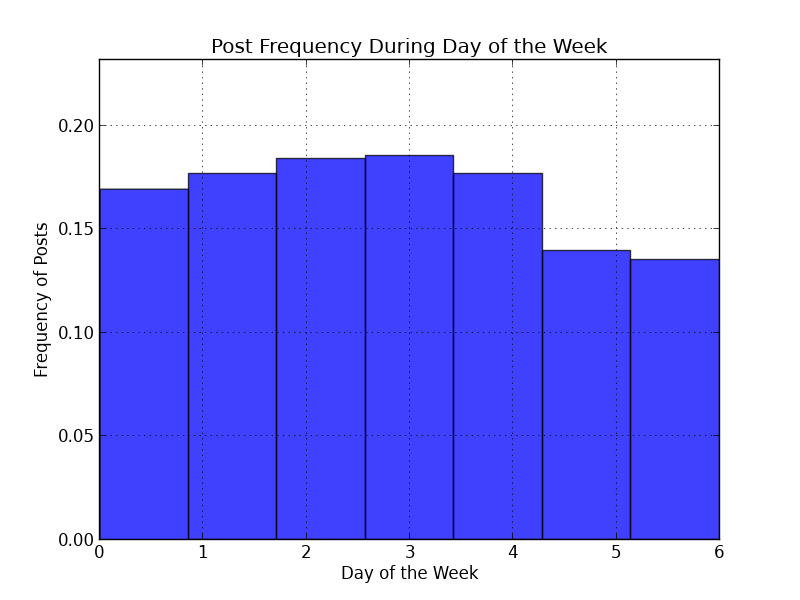
\includegraphics[width=\textwidth]{diagrams/daysofweek.png}
\caption{The daily post frequency. (Monday is 0)}
\label{fig:week_freq}
	\end{subfigure}
\end{center}
\end{figure}


This suggests that the \emph{time context} of which the posts were made are 
important when trying to determine the rate of posts.  As such, we factor in the 
day and hour information into our feature sets as well.

However, this time in stead of linear regression, we used a regression method 
known as Support Vector Regression (SVR), using a radial basis function kernel.  
This method allows the using of different kernels, allowing for better 
estimation of the target function.

The main focus of study in this report was to see if content helps with 
predicting thread updates would produce an improvement. Some of the ways that 
content data were extracted into feature vectors are the following: Word 
frequency, the tf-idf of these words, and Part-of-Speech tags.

We perform the standard preprocessing steps like removing stopwords and tokens 
of length less than three. We also use Porter's stemming algorithm as another 
preprocessing step, before performing a word frequency count. However, the use 
of the full vocabulary of the thread as a feature vector greatly increases the 
time needed to train the model. As such, we used a simple univariate regression 
technique for feature selection, and selected only the $K$ best tokens for 
consideration. Table \ref{table:vocab_exp} shows the results of this experiment.  
	
\begin{table}
	\footnotesize
\begin{center}
	\begin{tabular}{|l|c|c|c|c|c|c|c|c|}
	\hline
	\input{tables/vocab_exp}
	\hline
	\end{tabular}
\end{center}
	\caption{Experiment results: Varying vocabulary size}
	\label{table:vocab_exp}
\end{table}

These feature sets are used in different combinations, with different window 
sizes. The results will be seen in the next chapter.

The methods in this section use features extracted from the current window. A 
model is then trained using these extracted features in order to make a 
prediction. We take a look now at a two other novel methods that we developed.

\section{Discounted sum of previous instances}
 
Posts made further in the history of the thread may have an effect on when the 
latest posts arrive. The magnitude of this effect, however, may diminish over 
time.

Instead of having a finite window for which all posts (in said window) are 
treated equally, why not try to account for all previous posts, but weigh them 
accordingly: the earlier they were made, the less weightage on the prediction 
the post should have.

Following this intuition we used a discounted sum over previous posts' word 
frequency vector:
\[
	\X'_t = \X_t + \alpha \X'_{t-1}
\]
where $\X_t$ is the feature vector at post $t$. $\alpha$ is the \emph{discount 
factor} and satisfies $0 \leq \alpha < 1$.

This new feature vector $\X'_t$ will be used in the same way as before, 
instances of $\X'$ will be regressed with their $\dt$ values. As before, we will 
look at the results for this method in the next chapter.

Up till now, we have looked at methods that treat the model as static -- once 
trained, the model never gets updated during run time. However, this is 
unrealistic due to the fact that over time, different words are popular as a 
direct result of different topics in the real world being popular. In this case, 
these fluctuations may be due to new updates to firmware being released or newer 
models of, say, a stereo set.

\section{Stochastic Gradient Descent}
We also used stochastic gradient descent to estimate the function $f$.  However, 
during runtime, instead of using a static function, we continue to allow $f$ to 
vary whenever new posts and their update times are observed.

Having already attempted using linear regression for this purpose, we have found 
it unsuitable for $f$ to be estimated by a linear function. Such a linear 
function has often resulted in making a negative prediction, and sometimes an 
overly huge one, when given feature vectors that have previously never been 
observed. The function has to be somehow constrained such that the value 
returned never drops below 0, and never predicts something too huge such that 
many posts are missed.



Since $f(\X) > 0$, we used a scaled sigmoid function,
\[
	f(\X) = \frac{\Lambda-\lambda}{1 + e^{\weights \cdot \X}} + \lambda
\]
where $\Lambda$ and $\lambda$ are the scaling factors. This results in $f: 
\mathbb{R}^{|\X|}  \rightarrow (\lambda,\Lambda)$. Bounding the estimation 
function between $\lambda$ and $\Lambda$ allows us to restrict the prediction 
from becoming negative, or, becoming exceedingly huge. For our purposes, we set 
$\lambda = Q_3 + 2.5(Q_{3} - Q_{1})$, where $Q_n$ is the value at the $n$-th 
quartile. A visual interpretation of such a curve can be seen in Figure 
\ref{fig:scaled_sigmoid}.
\begin{figure}
\begin{center}
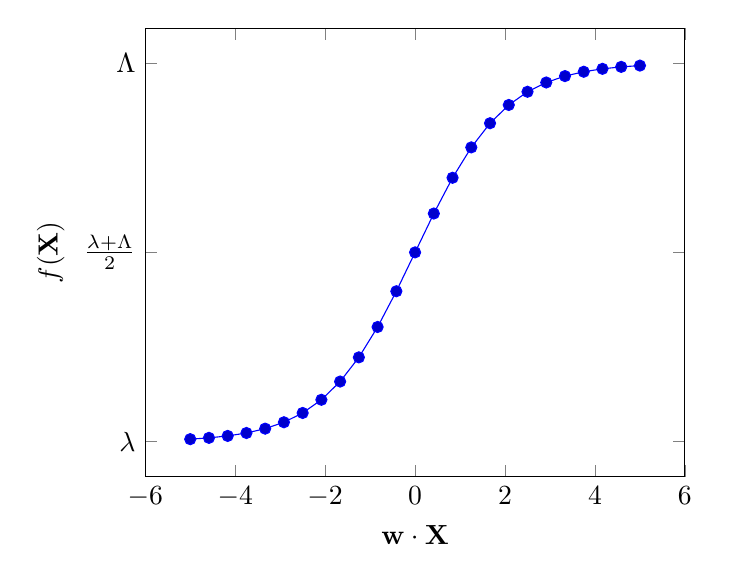
\begin{tikzpicture}
	\begin{axis}[
		xlabel=$\weights\cdot\X$,
		ylabel=$f(\X)$,
		ytick={0,0.5,1},
		yticklabels={$\lambda$,$\frac{\lambda + \Lambda}{2}$,$\Lambda$}
	]
\addplot {1/(1+ e^-x)}; \end{axis}
\end{tikzpicture}
\end{center}
\caption{Scaled sigmoid curve}\label{fig:scaled_sigmoid}
\end{figure}

The resulting update rule for $\weights$ is then given by,
\[
	\Delta \weights_i = \eta
				\underbrace{\left(\widehat{\dt} - \dt \right)}_{\text{error term}}
				\underbrace{\left( f(\X)(1-f(\X)) \right)}_{\text{gradient}}
						\X_i
\]
which is similar to the delta update rule found in artificial neural networks.  
We omit the scaling factor in the gradient as it is a constant and then 
experiment with various values of $\eta$, the learning rate. 

In this chapter, we have outlined the specific task we will be attempting, to 
try and predict the time from the current last post in the thread to the next.
We have discussed the types of features we will be using, time context features, 
with a focus on content features that consists mainly of the tokens present. We 
have also discussed the concept of a window, and how it could help to make 
predictions better. Also, two novel methods were discussed, and, in the next 
chapter, we will look at how these methods stack up against one another.

